%!TEX root = ../main.tex
\section{Restless rotting  bandits}
\label{sec:restless-model}
\subsection{Restless bandits model}
\subsubsection*{Feedback loop}
At each round $t$, an agent chooses an arm $i_t \in \possibleArms \triangleq \left\{ 1, ... , K\right\} $ and receives a noisy reward $o_t$. The reward associated to each arm $i$ is a $\subgaussian^2$-sub-Gaussian random variable with expected value of $\mu_i(t)$, which depends on the number of rounds $t$. Let $\historyt \triangleq \left\{ \left\{ i_s, o_s \right\}, \forall s < t \right\}$ be the sequence of arms pulled and rewards observed until round $t$, then 
%
\begin{equation}
\label{eq:restless-feedback}
o_{t} \triangleq \mu_{i_t}(t) + \noise_t
 \;\; \text{with}\; \EE{ \noise_t | \historyt }= 0 \;\; \text{and} \; \forall \lambda \in \R, \; \EE{ e^{\lambda\noise_t}} \leq e^{\frac{\subgaussian\lambda^2}{2}}.
\end{equation}
%

\subsubsection*{Objective}
We will only consider deterministic agents which output an arm $i$ at each round $t$. Like in the previous chapter, we distinguish offline (or oracle) policies~$\pi \in \PiO$ - which are functions which map the round $t$ and the set of reward functions to arms - from online (or learning) policies~$\pi \in \PiL$ - which are functions from the history of observations $\mathcal{H}_t$ at a round $t$ to arms. For both types of policies, we often use the shorter notation $\pi(t)$, where the dependency on $\mu$ or $\mathcal{H}_t$ is implicit. The performance of a policy $\pi$ is measured by the (conditionally expected) rewards accumulated over time, 
%
\begin{equation}
\label{eq:cumul-reward-restless}
J_T(\pi) \triangleq \sum_{t=1}^T \mu_{\pi(t)}\pa{t}.
\end{equation}
%

\begin{proposition}
The characterization of the optimal oracle policies is straightforward,
\[\pi^\star \in \argmax_{\pi \in \PiO} J_T(\pi) \iff \forall t \leq T,  \pi^\star(t) \in \argmax_{i \in \arms} \mu_i\pa{t}.\]
In the following, we call $i^\star_t \in \argmax_{i \in \arms} \mu_i\pa{t}$ one of the best arm at the round $t$, and $\mu_\star(t) \triangleq \max_{i \in \arms} \mu_i\pa{t}$ the corresponding best value.
\end{proposition}
Notice that there may be several optimal policies if, at a given round $t$, there are several arms with maximal value. However, all these policies get the same cumulative reward at every round; thus, the tie-break rule can be chosen arbitrary without impacting the performance.  We set a policy $\pi^\star\in \argmax_{\pi \in \PiO} J_T(\pi)$. Calling $J_T^\star = J_T(\pi^\star)$ the largest cumulative reward achievable, one can measure the regret of any policy (learning or oracle) compared to the optimal one, 
\begin{align}\label{eq:restless-regret}
\regret(\pi) \triangleq J^\star_T - J_T(\pi).
\end{align}
%
\begin{remark}
Like in the rested setup, the regret is measured against the optimal oracle policy rather than a fixed-arm policy as it is a case in adversarial bandits. Moreover, for constant $\mu_i(t)$-s, the problem, and definition of regret reduce to the ones of stationary stochastic bandits (where the regret is measured against the best fixed-arm policy which is also the optimal oracle policy). 
\end{remark}
%

\subsection{Piece-wise stationary bandits}
\label{subsec:piecewise}
\citet{garivier2011upper-confidence-bound} study the restless bandits case, where rewards are piece-wise stationary. 
 \begin{assumption}\label{assum:piece-wise}
Let $V$ be a positive constant and $\Upsilon_T$ a positive integer.  $\mu_i : \NN^\star \rightarrow [- V, 0]$\footnote{We could choose any interval $\left[x, x+V\right]$. Yet, with the upcoming decreasing assumption, choosing $[- V, 0]$ instead of $[0, V]$ emphasizes that the learner cannot infer parameter $V$ from the first pulls. Notice that we will never use that our rewards are negative in our analysis.} are piecewise stationary non-increasing functions of the time $t$ with at most $\Upsilon_T-1$ breakpoints. Formally, 
\[\sum_{t=1}^{T-1} \mathbbm{1}\left(\exists i\!\in\! \arms, \mu_i(t) \!\neq\! \mu_i(t\!+\!1)\right)\leq \Upsilon_T\!-\!1.\]
\end{assumption}
%
 We call $\left\{t_k\right\}_{k \leq \Upsilon-1}$ the set of breakpoints with $t_0 = 0$, $\mu_i^k$ the value of $\mu_i(t)$ for $t \in \left\{t_k+1 , \dots, t_{k+1}\right\}$. We call $i^\star_k \in \argmax_{i \in \arms}{\mu_i^k}$ (one of) the best arm in batch $k$, $\mu_\star^k \in \max_{i \in \arms}{\mu_i^k}$ the corresponding best value, and $\Delta_{i,k} \triangleq \mu_{\star}^k - \mu_i^k$ the gap to the best arm for arm $i$ during batch $k$.
%
\subsubsection{Lower Bounds}

\begin{proposition}[\citet{auer2002nonstochastic}]
\label{prop:piecewise_lb}
For any strategy $\pi$, there exists a $K$-armed piece-wise stationary bandit scenario with means $\{\mu_i(t)\}_{i,t}$ satisfying Assumption~\ref{assum:piece-wise} such that,
\[
    \mathbb{E}\left[R_T(\pi)\right] \geq \frac{\sigma}{32}\sqrt{ \Upsilon_T KT}\,.
\]
\end{proposition}

This bound is not surprising as it shows that piece-wise stationary bandits with $\Upsilon_T$ change-points are at least as hard as $\Upsilon_T$ stationary problems with horizon $\frac{T}{\Upsilon_T}$ \citep{auer2002nonstochastic}. We will show a slightly stronger result in Subsection~\ref{subsec:restless-rotting}.

\citet{garivier2011upper-confidence-bound} shows a self-bonding property of the regret. They build a problem $\mu'$ on which the reward function equals the reward on a stationary problem $\mu$ except on a period $\tau$ (see Figure~\ref{fig:garivier-lb}). During this time span, the best arm of $\mu$ keeps its value while the worst arm \textit{increases} to become optimal. The size of $\tau$ is chosen inversely proportional to the average pulling rate of the bad arm in $\mu$. Indeed, the lower the pulling rate of the bad arm, the longer the adversary can increase its value in $\mu'$ without being noticeable by the learner (which can be quantified thanks to Lemma~5.1, \citet{auer2002nonstochastic}). Since the pulling rate of the bad arm in $\mu$ is proportional to $R_T(\mu)$, we get a lower bound proportional to $\tau \sim \frac{T}{R_T(\mu)}$. We reproduce the version of the theorem in \citet{lattimore2020banditbook}. 

\begin{figure*}[h]
\centering
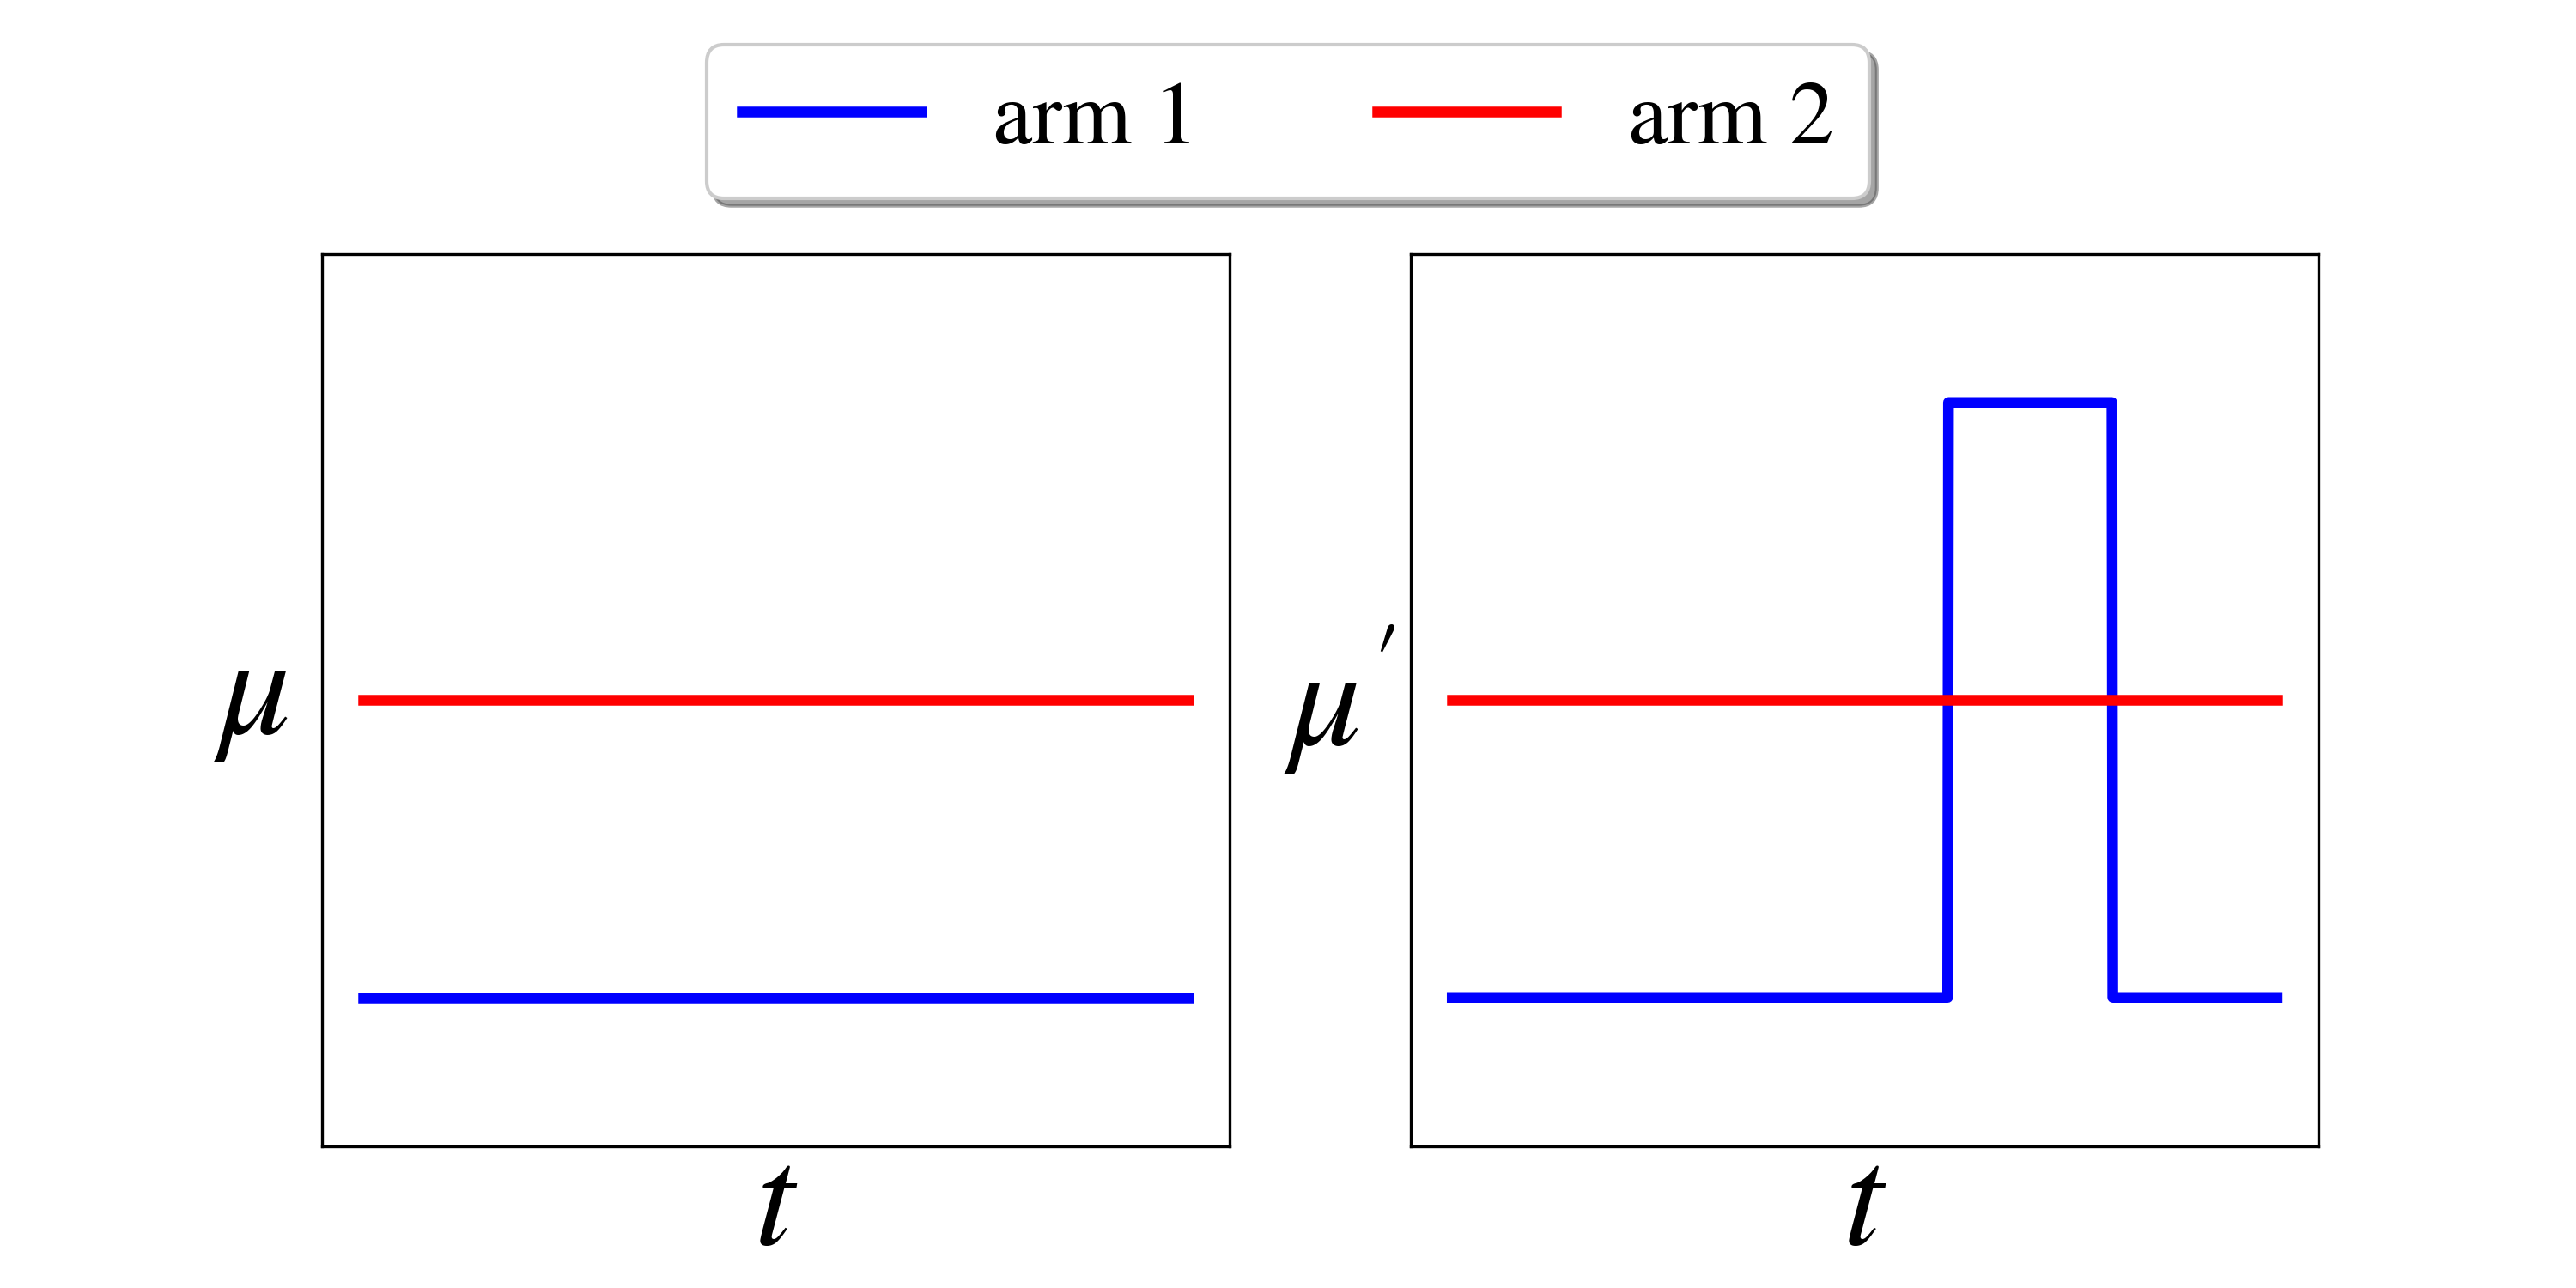
\includegraphics[clip, width= 0.99\textwidth]{2.2Restless/fig/garivier_lb.png}
\caption{The reward functions $\mu$ and $\mu'$. A policy with low regret on $\mu$ cannot achieve low regret on $\mu'$.}
\label{fig:garivier-lb}
\end{figure*}

\begin{proposition}[Theorem~31.2, \citet{lattimore2020banditbook}]
\label{prop:garivier-lb}
If a policy $\pi$ performs (in expectation) a regret $\EE{R_T(\pi, \mu)}$ on a 2-arm stationary instance $\mu$, one can find a piece-wise stationary instance $\mu'$ with only two breakpoints such that, for a sufficiently long horizon $T$, the regret is lower bounded by 
\[\EE{R_T(\pi, \mu')} \geq \frac{T}{22\EE{R_T(\pi, \mu)}}\,\cdot\]  
\end{proposition}

\begin{corollary}
\label{cor:garivier-lb}
Let $\pi$ a minimax optimal policy on the piece-wise stationary setups. Then, for a sufficiently large horizon $T$, there exists a universal constant $C$ such that for all the 2-arm stationary problems $\mu$, 
\[
\EE{R_T(\pi,\mu)} \geq C\sqrt{T}.
\]
\end{corollary}

These results state that one cannot have simultaneously a near-optimal problem-dependent regret rate $\cO\pa{\log{T}}$ on stationary instances and the minimax optimal piece-wise stationary rate $\cO\pa{\sqrt{T}}$. It is very different from the stationary case (or even with the rested rotting bandits presented in the last section) where some algorithms are shown to perform optimally both problem-dependent and problem-independent wise \citep{lattimore2018refining, menard2017klucb++}.

\subsubsection{Policies for piece-wise stationary bandits.}
\paragraph{Softmax policies.} For any sequence generated by an oblivious adversary, \EXPS \citep{auer2002nonstochastic} - an extension of \EXP - is guaranteed to achieve $\cO\pa{\sqrt{K\Upsilon_T T\log\pa{KT}}}$ regret against the best policy among the ones which change arms at most $\Upsilon_T -1$ times. The bound holds in the special case where the adversary generates the reward with noisy piece-wise stationary functions. In that case, the pseudo-regret definition is equivalent to the piece-wise stochastic regret defined in Equation~\ref{eq:restless-regret}. Indeed, the optimal policy is included in the set of $\cO\pa{\pa{KT}^{\Upsilon_T}}$ policies with at most $\Upsilon_T-1$ change of arms. 

\paragraph{Passive forgetting policies.} \DUCB \citep{kocsis2006discounted} and \SWUCB \citep{garivier2011upper-confidence-bound} are two ucb index policies which forget the older sample either by a discount factor or by a sliding window mechanism. The confidence interval increases when an arm has not been pulled for many rounds. When they are adequately tuned, these policies achieve respectively $\cO\pa{\sqrt{K\Upsilon_T T}\log{T}}$ and $\cO\pa{\sqrt{K\Upsilon_T T \log{T}}}$ minimax regret rate. While these policies do not improve the rate of \EXPS, they are deterministic and more explainable. 

\paragraph{Change-detection policies.} Instead of throwing away old samples at a fixed pace, one could remove samples from the index only when they notice a change in the arm's mean. This is the spirit of the Change-Detection ucb algorithms. These algorithms have three components: an ucb index, a change-detection subroutine, and a fixed active exploration rate (either deterministic or random pulls). The active exploration rate is meant to detect the arms which change from suboptimal value to optimal ones (like in Figure~\ref{fig:garivier-lb}). The optimal budget dedicated to active exploration scales with $\cO\pa{\sqrt{K\Upsilon_T T}}$. %When $\Upsilon_T$ is unknown, one can set a count $\Upsilon$ to $1$ and increases it at each detected change. 

\MUCB \citep{cao2019nearly} uses a simple change detector which compares the average of the last $\nicefrac{w}{2}$ samples with the average of the before last $\nicefrac{w}{2}$ ones and check whether the difference is significant or not. The optimal tuning of the parameter $w$ depends on the value of $\Upsilon_T$: if changes are large and frequent, one should choose a small value of $w$; if changes are small and sparse, one should choose a large value of $w$.

\CUSUMUCB \citep{liu2018change-detection} uses a change detector which constructs two random walks based on the upper and lower deviation of the new samples compared to the mean of the $M$ first ones. If one of the random walks reaches a threshold $h$, then the change detector triggers. The random walks are negatively biased with a small value $\epsilon$ to prevent the natural deviation to trigger the change detector. Again, the optimal value of the parameters $M$, $\epsilon$ and $h$ depends on the number of changes $\Upsilon_T$.

\GLRUCB \citep{besson2019generalized} uses the Gaussian Likelihood Ratio change detector. This change detector scans all the samples to detect any size of change on any period with high probability. The probability parameter only needs the knowledge of the horizon $T$ to achieve near-optimal minimax bound. \citet{mukherjee2019distribution} introduces a very similar algorithm but study the assumption where all the arms change their value significantly at each breakpoint. With this assumption, they do not need active exploration and recover problem-dependent bound $\cO\pa{\log{T}}$.

On the theoretical side, the analysis often assumes that each change is large enough to be detected before the next change. Indeed, after the detection of the breakpoint, they use the analysis of \UCB on each stationary batch. Before the change detection, they do not provide any non-trivial bound on the quality of the selected arm. 


\paragraph{Agnostic policies.}
\citet{auer2019adaptively} consider the problem with no assumption on the change-point detectability. They propose \ADSWITCH, which also uses a parameter-free change-detection subroutine but with an elimination policy: it pulls arms in a round-robin way in a refined set of good arms. Arms are excluded from this set when they demonstrate with high probability that they underperform. The bad arms are also actively explored with consecutive sampling: the algorithm selects at random an arm and a deviation size $\Delta$ and pulls the arm the right number of rounds to detect if there is a change of size $\Delta$ in the arm's value. \citet{chen2019new} extend this technique to the contextual bandits problem.

A previous attempt \citep{cheung2019new} to solve this problem uses an expert aggregation bandit algorithm (e.g. \EXPfour) to select between different tuning of \SWUCB . Yet expert aggregation of bandit algorithm is problematic \citep{agarwal2017corralling, besson2018aggregation}, and \citet{cheung2019new} has to run each copy by batch with full restart. This technique leads to a suboptimal rate $\tcO\pa{\sqrt{K \max\pa{\Upsilon_T, \sqrt{T}} T}}$.


\subsection{Variation budget bandits}
\label{subsec:variation}
\citet{besbes2014stochastic} introduce the limited variation budget bandits, a restless setting where at each round Nature can modify the reward value of any arm but with a limited total variation budget $V_T$ at the round $T$. 

\begin{assumption}
\label{assum:variation}
$\mu_i : \NN^\star \rightarrow [- V_T, 0]$ are functions of the time $t$ with $V_T$ a positive constant. Moreover, we have that 
\begin{equation}
\label{eq:defbudget}
    \sum_{t=1}^{T-1} \sup_{i \in \arms} |\mu_i(t+1) - \mu_i(t) | \leq V_T\,.
\end{equation}
\end{assumption}


\paragraph{Lower Bound}
\begin{proposition}[\citet{besbes2014stochastic}]
\label{prop:variation_lb}
For any strategy $\pi$, there exists a  variation budget bandit scenario with means $\{\mu_i(t)\}_{i,t}$ satisfying Assumption~\ref{assum:variation} with a budget $V_T \geq \sigma \sqrt{\frac{K}{8T}}$ such that
%
\[
    \mathbb{E}\left[R_T(\pi)\right] \geq \frac{1}{16\sqrt{2}} \pa{\sigma^2 V_T KT^2}^{1/3}.
\]
\end{proposition}

In the next section, we prove a stronger statement, using only non-increasing reward functions. Yet, there is no additional difficulty. While the two Assumptions~\ref{assum:piece-wise} and~\ref{assum:variation} leads to different regret rate (see Proposition~\ref{prop:piecewise_lb}), the proof (see e.g. Lemma~\ref{lemma:lb} in the next subsection) shows that there is a strong similarity between the two problems, at least from a minimax perspective.

\paragraph{Policies for variation budget bandits.}
Most of the algorithms presented for the piece-wise stationary case are also near-optimal for the variation budget case. Indeed, \citet{besbes2014stochastic} show that \EXPS also learns in the variation budget setup. They also present \REXP, an algorithm based on \EXP with periodic restart which recovers a similar guarantee than \EXPS. \citet{cheung2019new} and \citet{russac2019weighted} extend \SWUCB and \DUCB to the linear bandit setting with variation budget. \citet{chen2019new} proves that \ADSWITCH is also optimal in the variation budget setting. However, change-detection ucb algorithms are not proved to perform well in the variation budget setting. Indeed, their proofs use the proof of \UCB on each stationary batch. In the variation budget setup, there is no stationary batch, which makes these algorithms harder to analyze. 

\subsection{The restless rotting assumption}
\label{subsec:restless-rotting}
\begin{assumption}
\label{assum:restless_rotting}
Reward functions $\left\{\mu_i \right\}_i$ are non-increasing with $t$.
\end{assumption}
We use this Assumption in conjunction with Assumption~\ref{assum:piece-wise} or~\ref{assum:variation}.
\begin{remark}
\label{remark:budget}
With the rotting assumption, the variation budget assumption is very similar to the bounded assumption. Indeed, any set of decreasing functions $\mu_i : \NN^\star \rightarrow [- V, 0]$ satisfies Equation~\ref{eq:defbudget} with $V_T = KV$. Reciprocally, any set of functions satisfying Equation~\ref{eq:defbudget} with $\mu_i(1) \in [- V_T, 0]$ are bounded in $[- 2V_T, 0]$. 
\end{remark}

\paragraph{Lower bounds.} We show that our additional decreasing assumption does not change the minimax rates of the two settings. This is an adaptation of the proof of \citet{besbes2014stochastic} where we only use rotting functions.

\begin{restatable}{proposition}{restapiecewiselb}
\label{prop:piecewise_lb2}
For any strategy $\pi$, there exists a \underline{rotting} piece-wise stationary bandit scenario with means $\{\mu_i(t)\}_{i,t}$ \underline{satisfying Assumptions~\ref{assum:piece-wise} and~\ref{assum:restless_rotting}} with $\Upsilon_T\! \leq \!\pa{\!\frac{32V^2T }{K\sigma^2}\!}^{\!\nicefrac{1}{3}\!}\!$ such that,
\[
    \mathbb{E}\left[R_T(\pi)\right] \geq \frac{\sigma}{32}\sqrt{ \Upsilon_T KT}\,.
\]
\end{restatable}
\begin{restatable}{proposition}{restavariationlb}
\label{prop:variation_lb2}
For any strategy $\pi$, there exists a \underline{rotting} variation budget bandit scenario with means $\{\mu_i(t)\}_{i,t}$ \underline{satisfying Assumptions~\ref{assum:variation} and~\ref{assum:restless_rotting}} with a budget $V_T \geq \sigma \sqrt{\frac{K}{8T}}$ such that,
%
\[
    \mathbb{E}\left[R_T(\pi)\right] \geq \frac{1}{16\sqrt{2}} \pa{\sigma^2 V_T KT^2}^{\nicefrac{1}{3}}.
\]
\end{restatable}

The condition on $\Upsilon_T$ in Proposition~\ref{prop:piecewise_lb2} follows from the previous remark: if $V$ is too small compared to $\Upsilon_T$, then we have a budget constraint - with associated lower bound in Proposition~\ref{prop:variation_lb2} - rather than a breakpoint constraint.


\paragraph{Proof}
 Our proof builds a set of rotting piece-wise stationary problems with an evenly spaced set of $\Upsilon -1$ breakpoints. The adversary can choose the distance between arms $\Delta=\frac{1}{4} \sqrt{\frac{\sigma^{2} K \Upsilon}{2 T}}$ at the maximum such that the best arm is barely identifiable between two breakpoints (see Lemma~5.1, \citet{auer2002nonstochastic}). At each breakpoint, each arm's value decreases by $\Delta$ or $2\Delta$. Even if the set of breakpoints would be known, the learner does not know which arm is the best on each stationary part. Hence, in the worst case, she suffers at least the sum of the minimax regret of $\Upsilon$ stationary bandits problems with horizon $\frac{T}{\Upsilon}$, \textit{i.e.}  $\cO \pa{\sqrt{K\Upsilon T}}$. In the piece-wise stationary setting, we can simply identify $\Upsilon = \Upsilon_T$. In the variation budget setting, the adversary has a constraint over $\Upsilon \Delta = \frac{1}{4} \sqrt{\frac{\sigma^{2} K \Upsilon^3}{2 T}}=  \cO\pa{V_T}$. Hence, when the budget is limited, the adversary can choose up to $\Upsilon = \cO\pa{ T^{1/3}}$ breakpoints such that the suboptimal arms are "sufficiently" far from the best one (\textit{i.e} at $\Delta$). This dependence on $T$ leads to the increased regret rate of $\cO\pa{T^{\nicefrac{2}{3}}}$.
 
\begin{lemma}\label{lemma:lb}
Let $\Upsilon \in \left\{1,\dots, T\right\}$ and $\left\{\tau_k \triangleq \ceil{\frac{T}{ \Upsilon}} \text{ if } k \leq T \bmod{\Upsilon} \text{ else } \floor{\frac{T}{ \Upsilon}}\right\}_{k\leq \Upsilon}$. We call $t_k = \sum_{k'=1}^k \tau_{k'}$ and $t_0 = 0$.  Consider a family of piece-wise stationary bandits indexed by a vector $i^\star\in (\{0\}\cup \arms)^{\Upsilon}$ as follows: arm $i$ is a Gaussian distribution $\mathcal{N}\pa{\mu_i(t), \sigma}$ such that 
\[
\forall k \in \left\{0 , \dots, \Upsilon -1 \right\}, \ \forall t \in \left\{t_{k-1}+1,\dots, t_{k}\right\}, \ 
\mu_i(t) = 
\begin{cases}
-k \Delta \text{ if } i = i^\star_k\\
-(k+1)\Delta  \text{ else.}
\end{cases}
\]
We denote by $\EEempty_{i^\star}$ the expectation under the problem indexed by $i^\star$. Then, if $\Delta = \frac{1}{4}\sqrt{\frac{\sigma^2K\Upsilon}{2T}}$, for any policy $\pi$ :
\[
 \exists i^\star\in (\{0\}\cup \arms)^{\Upsilon}, \  \EEempty_{i^\star}\big[R_T(\pi)\big]  \geq  \frac{\sqrt{\sigma^2KT\Upsilon}}{32}\cdot
\]
\end{lemma}
\begin{proof}
Note that when $i^\star_k = 0$ then all the arms share the same means. We also define the vector $i^\star_{-k}$ equals to $i^\star$ with the coordinate $k$ empty and for $i\in\arms$ the vector $(i^\star_{-k},i)$ as the vector where we fill the empty coordinate with $i$.  We fix a policy $\pi$ and we will lower bound its average regret on the bandits problem indexed by $i^\star \in \arms^\Upsilon$ 
\begin{align*}
    \frac{1}{K^{\Upsilon}} \sum_{i^\star\in \arms^{\Upsilon}}  \EEempty_{i^\star}\big[R_T(\pi)\big] &= \frac{1}{K^{\Upsilon}} \sum_{i^\star\in \arms^{\Upsilon}} \sum_{k=1}^{\Upsilon}\Delta \EEempty_{i^\star}[\tau_k - N_{i^\star_k}^k] \\
    &=\Delta \left(T - \frac{1}{K^{\Upsilon}} \sum_{i^\star\in \arms^{\Upsilon}} \sum_{k=1}^{\Upsilon} \EEempty_{i^\star}[N_{i^\star_k}^k]\right),
\end{align*}
where $N_i^k$ is the number of pulls of arm $i$ during epoch $k$. Thus we need to upper bound the following quantity
\[
\frac{1}{K^{\Upsilon}} \sum_{i^\star\in \arms^{\Upsilon}} \sum_{k=1}^{\Upsilon} \EEempty_{i^\star}[N_{i^\star_k}^k] = \sum_{k=1}^{\Upsilon} \frac{1}{K^{\Upsilon-1}} \sum_{i^\star_{-k}\in \arms^{\Upsilon-1}}\frac{1}{K} \sum_{i=1}^K\EEempty_{(i^\star_{-k},i)}[N_{i}^k]\,.
\]
Using the contraction of the entropy for the bounded random variable $N_{i}^k/\tau_k$ then the Pinsker inequality (see \citet{garivier2018explore}) we get
\[
2\left(\frac{1}{\tau_k K} \sum_{i=1}^K\EEempty_{(i^\star_{-k},i)}[N_{i}^k] -\frac{1}{\tau_k K} \sum_{i=1}^K\EEempty_{(i^\star_{-k},0)}[N_{i}^k] \right)^2 \leq \frac{1}{K} \sum_{i=1}^K \EEempty_{(i^\star_{-k},0)}[N_{i}^k] \frac{\Delta^2}{2\sigma^2}\CommaBin
\]
since problems $(i^\star_{-k},i)$ and $(i^\star_{-k},0)$ differ only by a gap $\Delta$ on the arm $i$ during epoch $k$. Thanks to the fact that  $\sum_i N_i^k \leq \tau_k$ we get 
\[
\frac{1}{K} \sum_{i=1}^K\EEempty_{(i^\star_{-k},i)}[N_{i}^k] \leq \frac{\tau_k}{K} + \frac{\Delta}{2\sigma \sqrt{K}}\tau_k^{\nicefrac{3}{2}}\,.
\]
Putting all together we have for $K\geq 2$
\begin{align*}
    \frac{1}{K^{\Upsilon}} \sum_{i^\star\in \arms^{\Upsilon}}  \EEempty_{i^\star}\big[R_T(\pi)\big]  \geq \left(\frac{T}{2} -  \sum_{k=1}^{\Upsilon} \frac{\tau_k^{\nicefrac{3}{2}} \Delta}{2\sigma \sqrt{K}}\right)\Delta\,.
\end{align*}
We have $\tau_k= \floor{\frac{T}{\Upsilon}}$ or $\tau_k= \ceil{\frac{T}{\Upsilon}}$  such that $\sum_{k=1}^{\Upsilon} \tau_k=T$. Hence, we have that $\tau_k \leq 2T/\Upsilon$ which leads to 
\[
 \frac{1}{K^{\Upsilon}} \sum_{i^\star\in \arms^{\Upsilon}}  \EEempty_{i^\star}\big[R_T(\pi)\big]  \geq  \left(\frac{1}{2}T - \frac{\sqrt{2}T^{\nicefrac{3}{2}}\Delta}{\sigma \sqrt{K\Upsilon}}\right)\Delta\,.
\]

Choosing $\Delta = \frac{1}{4}\sqrt{\frac{\sigma^2K\Upsilon}{2T}}$, we get 
\[
 \frac{1}{K^{\Upsilon}} \sum_{i^\star\in \arms^{\Upsilon}}  \EEempty_{i^\star}\big[R_T(\pi)\big]  \geq  \frac{1}{4}\sqrt{\frac{\sigma^2K\Upsilon}{2T}}\left(\frac{1}{4}T\right) \geq \frac{\sqrt{\sigma^2KT\Upsilon}}{32}\cdot
\]
We can conclude by noticing that the average expected regret across the problem set is lesser or equal to the maximum across the same problem set.
\end{proof}

\begin{proof}[Proof of Proposition~\ref{prop:piecewise_lb2}]
This result directly follows from Lemma~\ref{lemma:lb} by choosing $\Upsilon = \Upsilon_T$. Indeed, the set of problems $\left\{i^\star \in \left(\left\{0\right\} \cup \arms\right)^{\Upsilon_T} \right\}$ satisfy Assumptions~\ref{assum:piece-wise} and~\ref{assum:restless_rotting} as soon as $\Upsilon_T\Delta \leq V$, \ie $\Upsilon_T \leq \pa{\frac{32V^2T }{K\sigma^2}}^{\nicefrac{1}{3}}$.
\end{proof}


\begin{proof}[Proof of Proposition~\ref{prop:variation_lb2}]
\sloppy
We want to use Lemma~\ref{lemma:lb} but we need to make the set of problems $\left\{i^\star \in \left(\left\{0\right\} \cup \arms\right)^{\Upsilon_T} \right\}$ comply with Assumption~\ref{assum:variation}. First, the function are bounded by $-V_T$. Hence, we need : 
\begin{equation}
\label{eq:bounded_condition}
  \Upsilon \Delta \leq V_T.  
\end{equation}

Second, the total variation is bounded according to Equation~\ref{eq:defbudget}. When $t$ is not a breakpoint, the variation is null. At each breakpoint, the maximal variation across the arm is $2\Delta$. For $\Upsilon-1$ breakpoint, we have that 


\begin{equation}
\label{eq:totalvar_condition}
  2\Delta \pa{\Upsilon-1}  \leq V_T.  
\end{equation}

Since $ 2\Delta \pa{\Upsilon-1} \leq \frac{\sigma}{2}\sqrt{\frac{K}{2T}}\Upsilon^{\nicefrac{3}{2}} $, we choose 
\begin{equation}
\label{eq:set_upsilon}
\Upsilon = \min\pa{\max\pa{\floor{ 2\left(\frac{V_T^{2}T}{K\sigma^{2}}\right)^{\nicefrac{1}{3}}},1},T}.
\end{equation}

By construction, \ref{eq:set_upsilon} satisfies \ref{eq:totalvar_condition}. Moreover, when $\Upsilon >1$, \ref{eq:totalvar_condition} is more restrictive than \ref{eq:bounded_condition}. For $\Upsilon = 1$, we simply assume $\Delta \leq V_T$, \textit{i.e.} $V_{T} \geq \sigma \sqrt{\frac{K}{8 T}}$.

Plugging \ref{eq:set_upsilon} in Lemma~\ref{lemma:lb} allows us to conclude 
\[
    \mathbb{E}\left[R_T(\pi)\right] \geq \frac{1}{16\sqrt{2}} V_T^{\nicefrac{1}{3}}\sigma^{\nicefrac{2}{3}}K^{\nicefrac{1}{3}}T^{\nicefrac{2}{3}}.
\]
\end{proof}